\documentclass[Report.tex]{subfiles}
\begin{document}
When creating visualizations it is not always enough with one idiom to present the data in an understandable way. One way to cram more information into the idiom, but still keeping the number of variables low is, to either manipulate the view of the idiom or to facet into multiple idioms. 
\subsubsection{View Manipulation}
By creating multiple views in an idiom, the idiom can contain more information, without introducing clutter. The different views can include changes like switching between different idioms, changing the viewpoint, changing the order of the data, changing the number of items shown and so on. For example one can change the way the data is ordered by sorting the data by different variables. This is very powerful because of spatial position being the highest ranked visual channel. Many view manipulations are based on animation. Animating has a trade off, the cognitive load can be very high if too many elements change. This means that we get low cognitive load if either some elements are static and others are moving, or some groups of elements are static and others are moving. If few elements change by a graduate transition, the viewer can keep the context between the two views. \cite[Chapter 11]{Tamara}

Selecting one or more elements is common in many interactive visualizations. The result of selecting an element is then some change in the view. It has to be considered which elements the user can select, and how many. Choosing how to select items is also a subject which has to be considered, clicking to select, hovering over some element with the cursor or something else. 
Changing the view by highlighting some element and creating pop out could be done by changing the channel, for example the color, the size, the outline or the shape of the element. This change should of course be so dramatic that the element clearly stands out from the rest. Look at Figure \ref{fig:highlighted} for an example of highlighting. \cite[Chapter 11]{Tamara}
\begin{figure}
\center
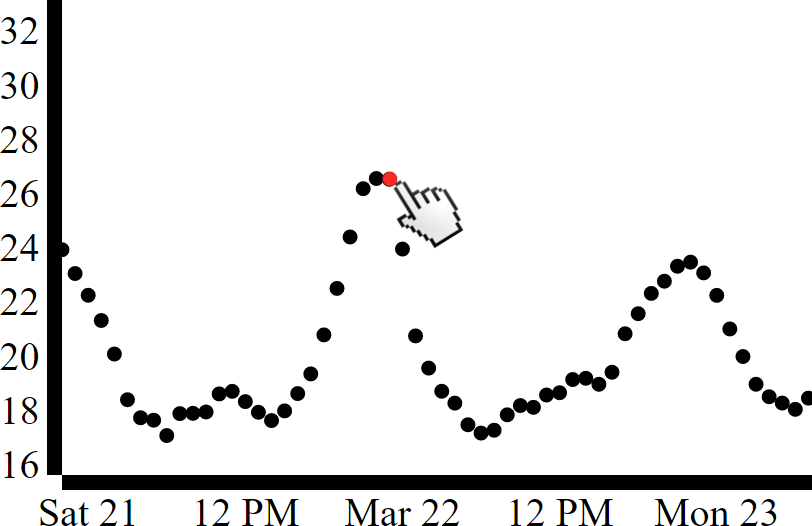
\includegraphics[scale=.4]{Highlighted}
\caption{Highlighting the selected element}
\label{fig:highlighted}
\end{figure}

Another option for an interactive idiom is the ability to navigate the view by changing the viewpoint. Here we think as if we have a camera pointed at the view. We can then change the view by zooming, panning or rotating the the camera around its own axis. There are two kinds of zooming, geometric zooming and semantic zooming. Geometric zooming is straight forward making some elements appear closer to the camera. With semantic zooming not only the size of the elements change, but the semantics too. Semantic zooming changes what is shown, and possibly the representation of it. For example zooming semantically could reveal more detail about some element showing new information about it.
Navigation could also be changed through reduction of attributes, by slicing, cutting or projecting. These are all dimension reduction techniques. To slice, a specific value at a dimension is chosen, and only elements matching this value is shown. A cut is made by placing a plane in front of the camera, all elements in front of the plane is not shown, in this way it is possible to explore elements behind other elements, or look inside 3D objects. Projection is done by eliminating some dimension while still showing all the data. This is similar to what the humans do when looking at a 3D object.
\subsubsection{Facet}
Faceting is splitting the view up into multiple views or into multiple layers. One of the main reasons to facet is to compare views. This is much easier than comparing two views in a changing view, because we do not have to remember the prior view, but just move our eyes to compare them. Another reason to facet is to gain more information about the data through a multiform design, where data is shown using different encodings. By having multiple views, more attributes can also be shown. Of course when one has multiple views shown beside each other, each view has less space, which is one of the trade-offs and why having multiple layers on top of each other, and switching between them sometimes is better. When having juxtaposed views it might be interesting to link the views.  This could be done by sharing the data, sharing the visual encoding, synchronizing the navigation or highlighting. 

Each view could show different subsets of the data, or having different viewpoints like the classic overview in one view  combined with detail in another view. 
Multiple views sharing encoding but showing different parts of the data, is called \emph{small multiples} and is often structured in a matrix. This could be an alternative to animations, where we lay out all the frames. The cognitive load is smaller with small multiples, and it is easy to go one frame back or forth. An example of small multiples is seen in Figure \ref{fig:smallmultiples}.
\begin{figure}
\center
\includegraphics[scale=0.3]{"Small multiples"}
\caption{An example of small multiples}
\label{fig:smallmultiples}
\end{figure}
Instead of juxtaposing the views, it is an option to stack them into a single frame. The views should have the same horizontal and vertical extend and blend together as one frame, by being transparent where there are no marks. The problem with stacking is distinguishing between the layers. This is easy with only a few layers, especially if the layers use different visual channels. But distinguishing between more than three layers, can be a real challenge. \cite[Chapter 12]{Tamara}

\end{document}